\documentclass[11pt,a4paper]{ctexart}
\usepackage{fontspec}
\defaultfontfeatures{Mapping=tex-text}
\usepackage{xunicode}
\usepackage{xltxtra}
%\setmainfont{???}
\usepackage{amsmath}
\usepackage{amsfonts}
\usepackage{amssymb}
\usepackage{graphicx}
\usepackage{amsthm}
\usepackage{array}
\usepackage{float}   %{H}
\usepackage{booktabs}  %\toprule[1.5pt]
\usepackage[titletoc]{appendix}
\usepackage{tcolorbox} %彩色框框
%===================%插入代码需要的控制
\usepackage{listings}
\usepackage{xcolor}
\setmonofont{Consolas}%字体
\lstset{
	numbers=left, 
	numberstyle= \tiny, 
	keywordstyle= \color{ blue!70},
	commentstyle= \color{red!50!green!50!blue!50}, 
	frame=shadowbox, % 阴影效果
	rulesepcolor= \color{ red!20!green!20!blue!20} ,
	escapeinside=``,% 英文分号中可写入中文
	breaklines=true,
	basicstyle=\ttfamily 
} 
%===================%
\usepackage[left=2cm,right=2cm,top=2cm,bottom=2cm]{geometry}

\newtheorem{theorem}{定理}
\newtheorem{definition}{定义}
\newtheorem*{solution}{解}

\title{定性数据统计分析作业 (6)}
\author{钟瑜 \quad 222018314210044}
\date{\today}
\begin{document}
\maketitle
\pagestyle{plain}%设置页码
%================================================================%
\begin{figure}[H]
	\centering
	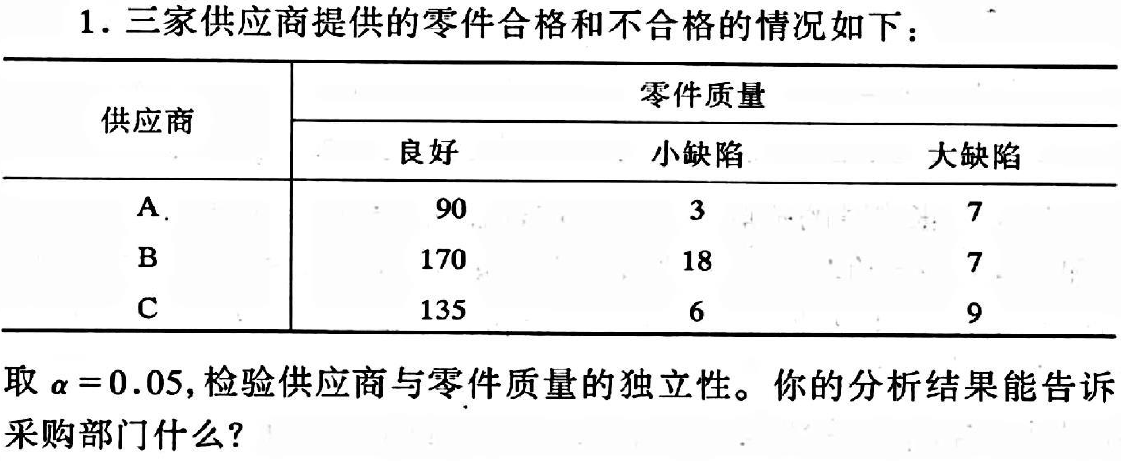
\includegraphics[width=0.7\textwidth]{screenshot001}
	\label{fig:screenshot001}
\end{figure}
\begin{solution}
\end{solution}
\begin{lstlisting}[language=r]
> x<-matrix(c(90,170,135,3,18,6,7,7,9),nrow=3)
> chisq.test(x,correct = F)

Pearson's Chi-squared test

data:  x
X-squared = 7.7117, df = 4, p-value = 0.1027
\end{lstlisting}
p值大于$ \alpha $=0.05,故接受原假设,认为供应商与零件质量独立,即选哪个供应商,其质量都差不多\\
%=======================================================
\begin{figure}[H]
	\centering
	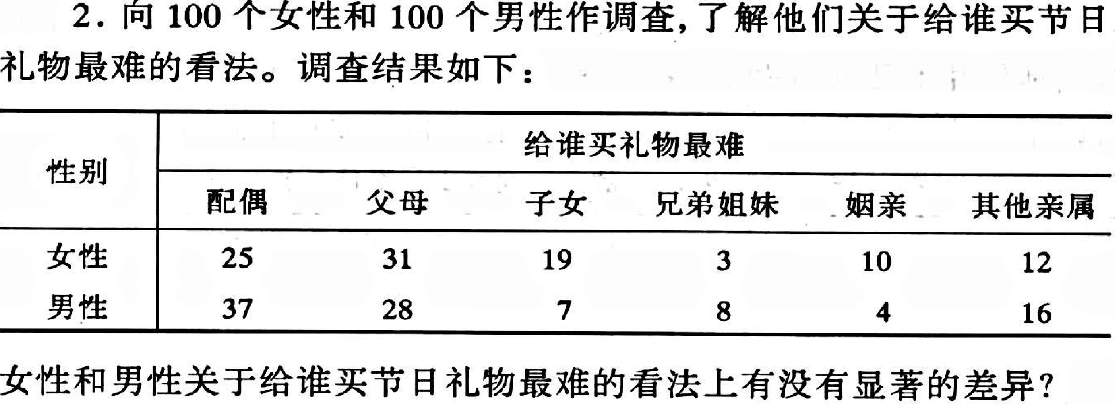
\includegraphics[width=0.7\textwidth]{screenshot002}
	\label{fig:screenshot002}
\end{figure}
\begin{solution}
\end{solution}
\begin{lstlisting}[language=r]
> x2<-matrix(c(25,37,31,28,19,7,3,8,10,4,12,16),nrow=6)
> chisq.test(x2,correct = F)

Pearson's Chi-squared test

data:  x2
X-squared = 32.927, df = 5, p-value = 3.892e-06
\end{lstlisting}

p值于小$ \alpha $=0.01,故不接受原假设,认为女性和男性关于给谁买节日礼物最难的看法上有显著差异.\\
%=======================================================
\begin{figure}[H]
	\centering
	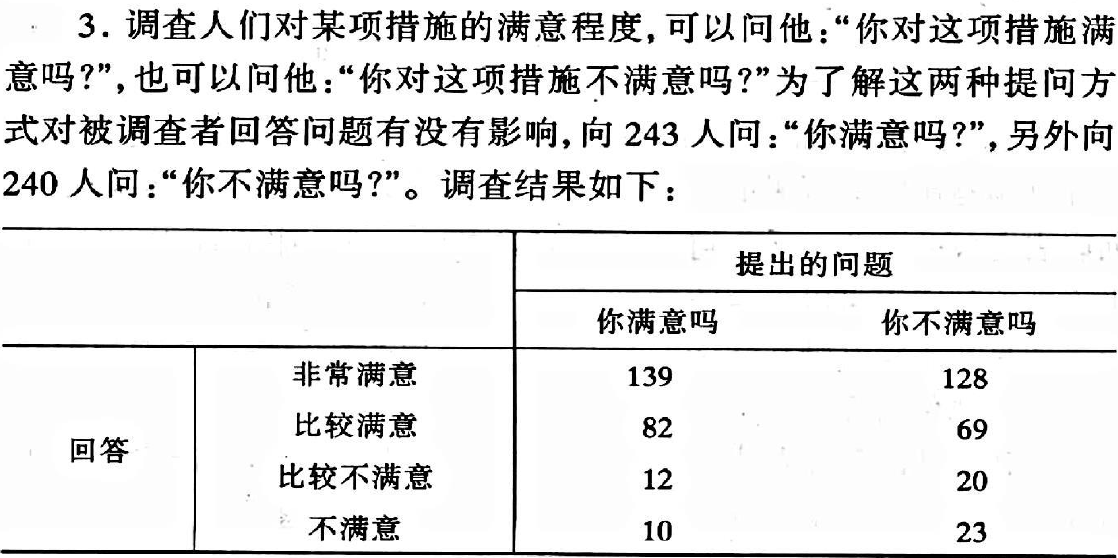
\includegraphics[width=0.7\textwidth]{screenshot005}
	\label{fig:screenshot005}
\end{figure}
\begin{figure}[H]
	\centering
	
\includegraphics[width=0.7\textwidth]{screenshot003}
	\label{fig:screenshot003}
\end{figure}
\begin{solution}
\end{solution}
\begin{lstlisting}[language=r]
> x3<-matrix(c(139,82,12,10,128,69,20,23),nrow=2)
> chisq.test(x3,correct = F)

Pearson's Chi-squared test

data:  x3
X-squared = 5.705, df = 3, p-value = 0.1269
\end{lstlisting}

p值大于$ \alpha $=0.01,故接受原假设,认为这两种提问方式被调查者回答问题没有影响.\\

%======================================================
\begin{figure}[H]
	\centering
	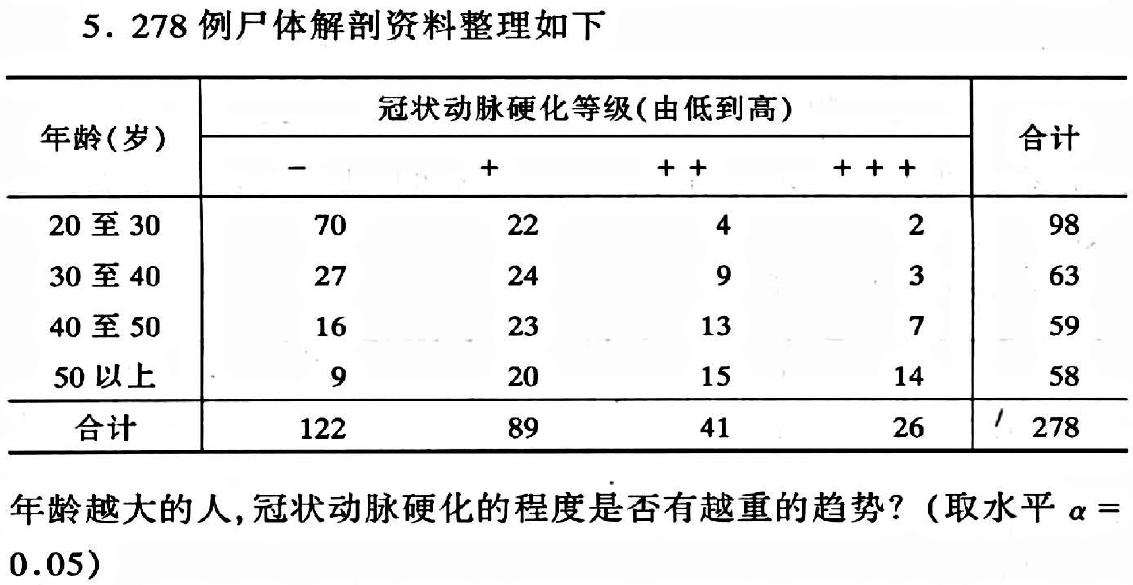
\includegraphics[width=0.7\textwidth]{screenshot007}
	\label{fig:screenshot007}
\end{figure}
\begin{solution}
\end{solution}
\begin{lstlisting}[language=r]
> congruence_test=function(x,alternative="twoside")
+     #适用于列联表的相合性检验问题
+     #x为列联表矩阵;alternative对应于备择假设
+ {
+     n=sum(x)
+     G=0;H=0
+     r=nrow(x)
+     c=ncol(x)
+     r1=r-1;c1=c-1
+     for (i in 1:r1){
+         for (j in 1:c1){
+             G=G+x[i,j]*sum(x[(i+1):r,(j+1):c])
+         }
+     }
+     for (i in 1:r1){
+         for (j in 2:c){
+             H=H+x[i,j]*sum(x[(i+1):r,1:(j-1)])
+         }
+     }
+     z=G-H
+     TA=sum(rowSums(x)*(rowSums(x)-1)/2)
+     TB=sum(colSums(x)*(colSums(x)-1)/2)
+     #TAB=G+H+TA+TB-n*(n-1)/2
+     Cn2=n*(n-1)/2
+     #计算各系数的值
+     Kendall_TAO=z/sqrt((Cn2-TA)*(Cn2-TB))
+     Gamma=(G-H)/(G+H)
+     d_BA=(G-H)/(Cn2-TA)
+     d_AB=(G-H)/(Cn2-TB)
+     
+     #近似公式,表示sigma的平方
+     sigma_2=(n^3-sum(rowSums(x)^3))*(n^3-sum(colSums(x)^3))/(9*n^3) 
+     
+     #构建U统计量
+     U=z/sqrt(sigma_2)
+     if(alternative=="twoside")
+     {p_value=1-pchisq(U^2, 1)}
+     else 
+     {
+         if(alternative=="greater")
+         {p_value=pnorm(-U)}
+         else if(alternative=="less")
+         {p_value=pnorm(U)}
+         else{cat("please input:\n alternative= 'twoside','greater',or'less'")}
+     }
+     cat('【各种相关系数】\n')
+     cat('Kendall_TAO=',Kendall_TAO,'\n')
+     cat('Gamma=',Gamma,'\n')
+     cat('d_BA=',d_BA,'\n')
+     cat('d_AB=',d_AB,'\n\n')
+     cat('【相合性检验】\n')
+     cat('U检验统计量的值',U,'\n')
+     cat('p_value=',p_value)
+ }

> congruence_test(x5)
【各种相关系数】
Kendall_TAO= 0.4245224 
Gamma= 0.5719659 
d_BA= 0.4064291 
d_AB= 0.4434212 

【相合性检验】
U检验统计量的值 8.292197 
p_value= 1.110223e-16
\end{lstlisting}
p值小于$ \alpha $=0.01,故拒绝原假设,认为年龄越大的人,冠状动脉硬化的程度有越重的趋势.\\

\end{document}